\section{Wyniki i analiza pomiarów}


% Tabela z pomiarami
\begin{table}[!ht]
    \centering
    \begin{tabular}{|c|c|c|c|c|c|}
    \hline
    Temperatura & Próbka 1 & Próbka 2 & Próbka 3 & Próbka 4 \\ \hline
    $^{\circ}C$ & $\Omega$ & $k\Omega$ & $\Omega$ & $\Omega$ \\ \hline\hline
    100         & 146.7    & 1.004     & 40.5     & 8.6  \\ \hline
    95          & 146.6    & 1.013     & 42       & 9    \\ \hline
    90          & 145.9    & 1.08      & 45       & 9.7  \\ \hline
    85          & 144.8    & 1.173     & 48.9     & 10.6 \\ \hline
    80          & 143.7    & 1.268     & 52.5     & 11.4 \\ \hline
    75          & 141.9    & 1.406     & 58.4     & 12.8 \\ \hline
    70          & 140      & 1.588     & 64.9     & 14.2 \\ \hline
    65          & 137.8    & 1.834     & 73.7     & 16.3 \\ \hline
    60          & 135.2    & 2.178     & 86       & 19.4 \\ \hline
    55          & 132.4    & 2.59      & 100.4    & 22.9 \\ \hline
    50          & 130.3    & 3.149     & 119.5    & 27.8 \\ \hline
    45          & 128.5    & 3.689     & 139.4    & 33.2 \\ \hline
    40          & 126      & 4.64      & 168.9    & 48   \\ \hline
    35          & 122.5    & 6.02      & 215.6    & 53.4 \\ \hline
    30          & 116.4    & 10.56     & 343.8    & 88.5 \\ \hline
    \end{tabular}
    \caption{Tabela dokonanych pomiarów dla 4 różnych próbek}
    \label{tab:my_label}
\end{table}

Z zebranych danych ustaliliśmy, że próbka nr. 1 była wykonana z metalu, natomiast próbki 2, 3 oraz 4 z materiału półprzewodnikowego.

Do dalszej analizy wybraliśmy próbkę nr.1 oraz nr.2.

\newpage
\subsection{Próbka nr.1 - metal}

\begin{figure}[!ht]
    \centering
    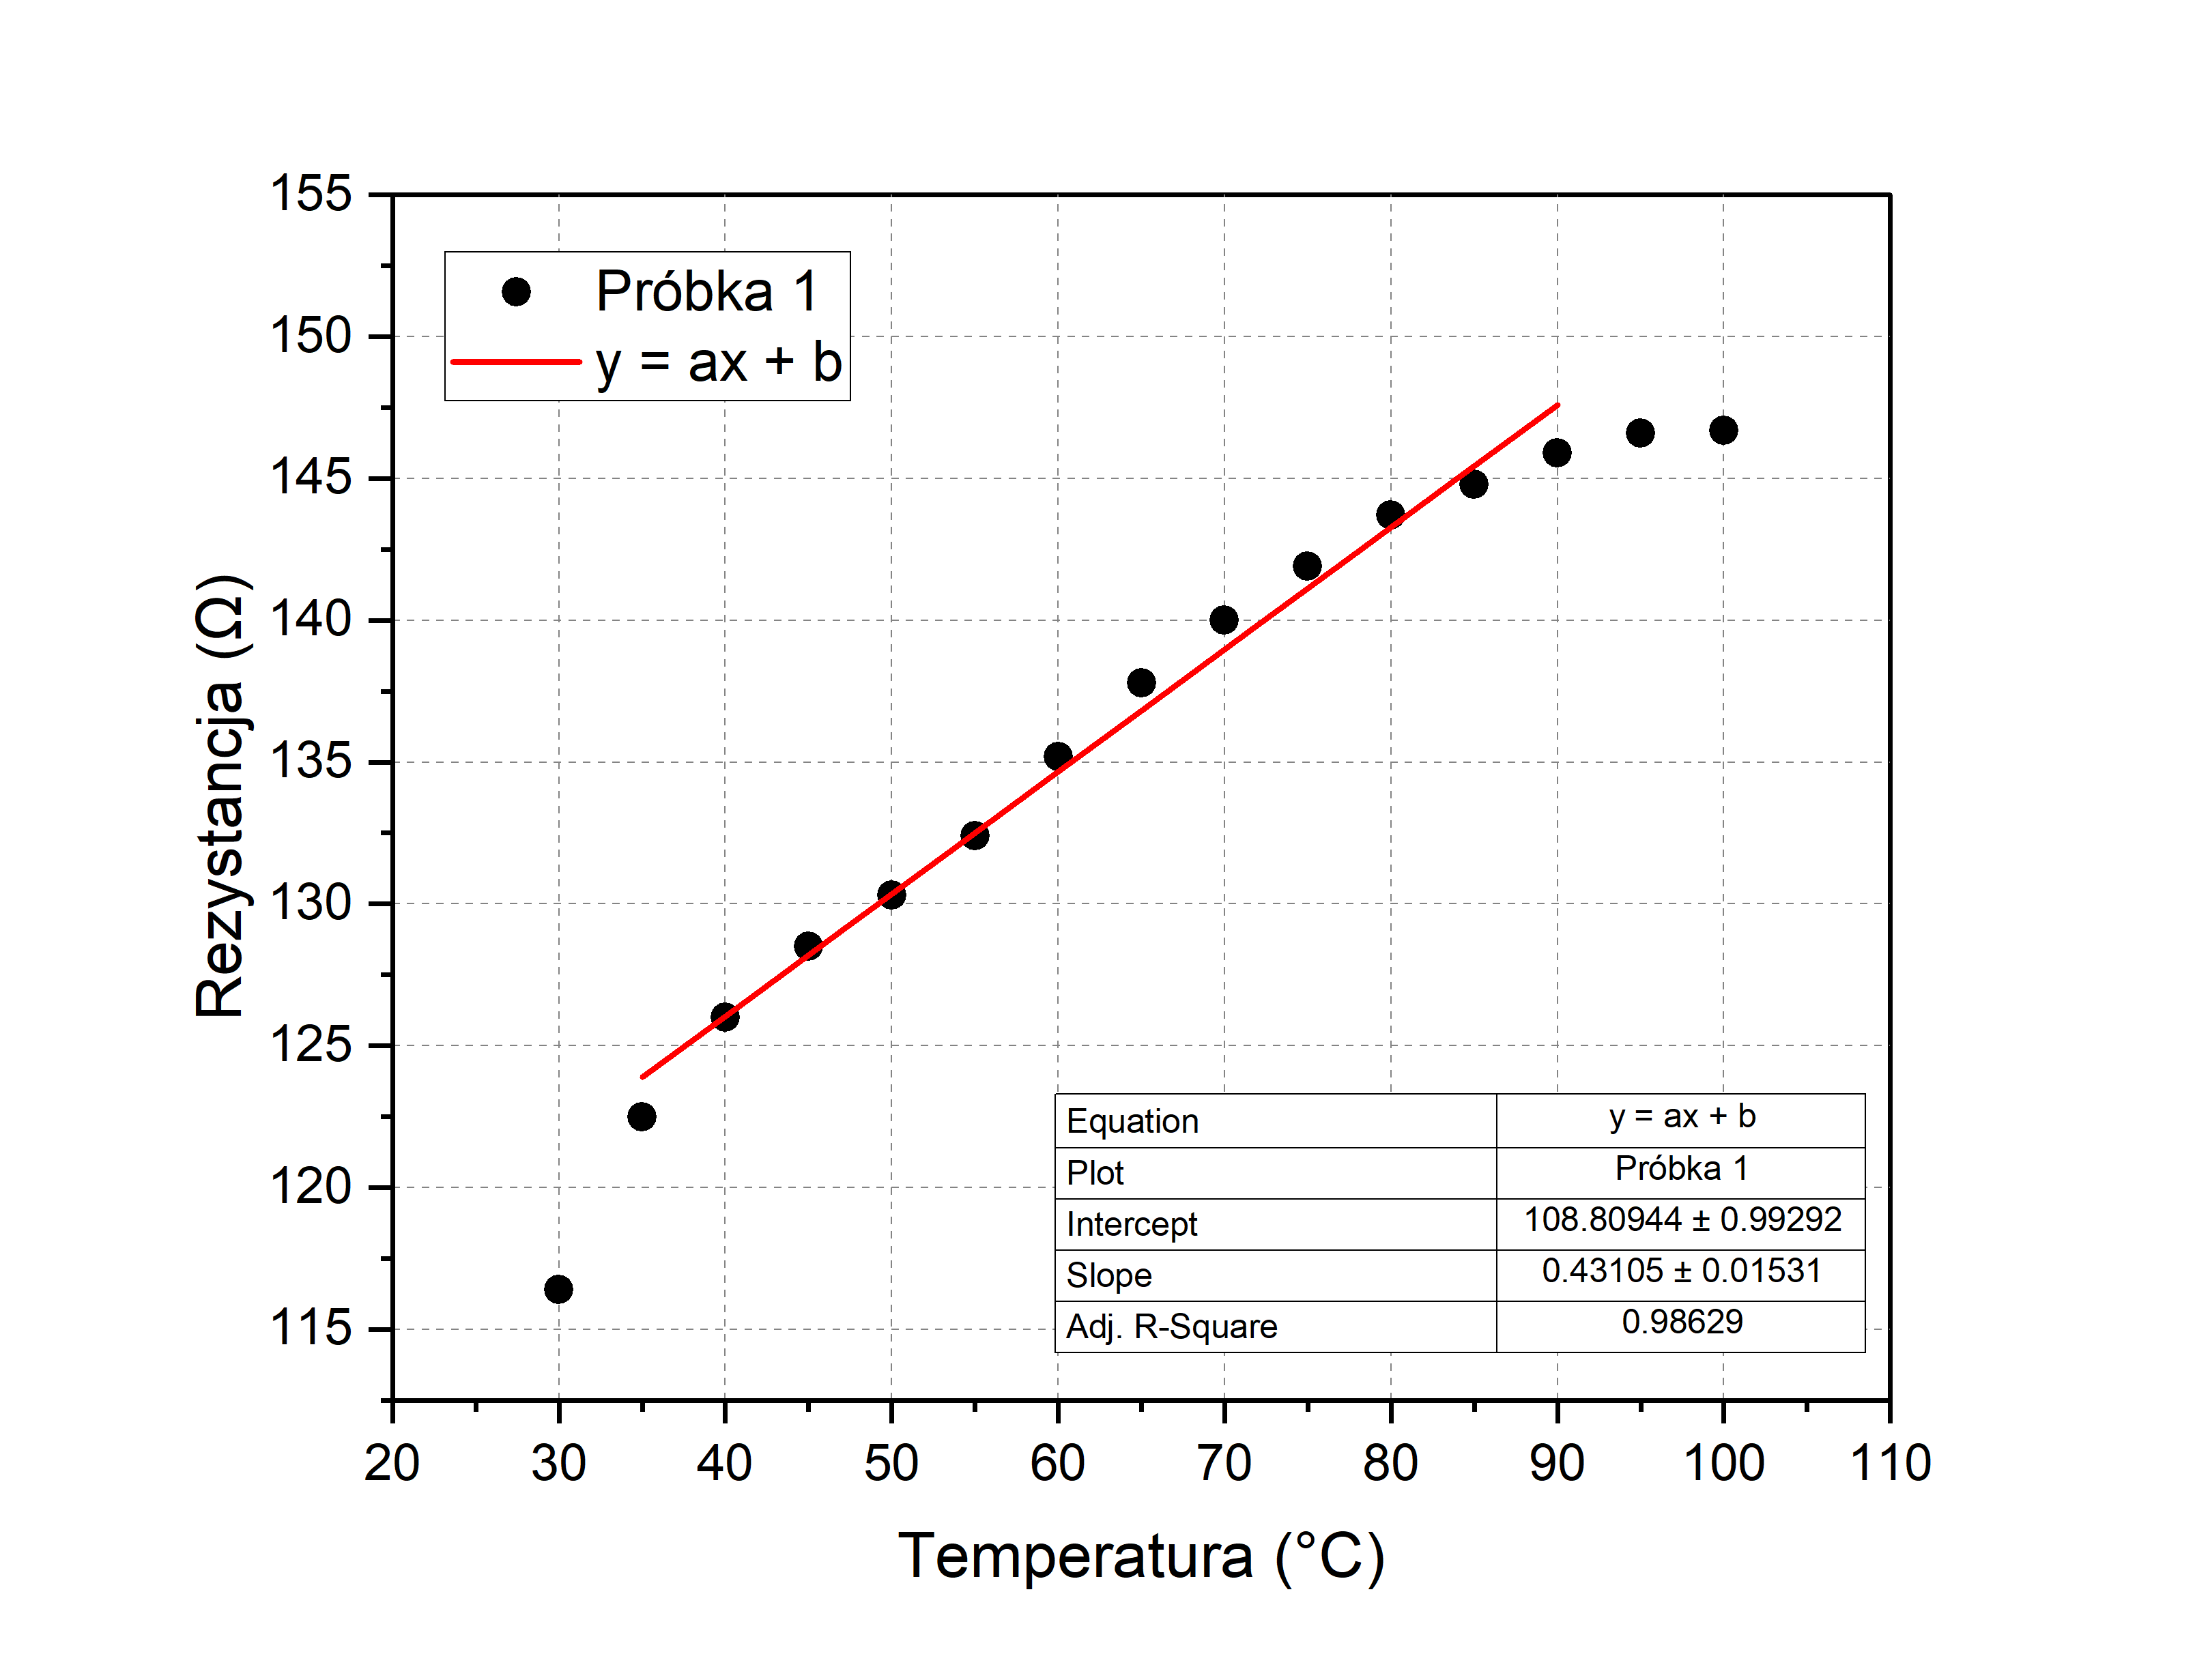
\includegraphics[width = 150mm]{imgs/Graph1.png}
    \caption{Wykres zależności $R_m = f(t)$ dla próbki nr.1}
    \label{fig:metal}
\end{figure}

Po stworzeniu wykresu zależności $R_m = f(t)$ spodziewaliśmy się funkcji liniowej.
Brak spodziewanego wyniku mówi nam, że na krańcach przedziału danych doszło do błędu pomiarowego. Najprawdopodobniej był to błąd ludzki.
W związku z tym dopasowaliśmy regresję liniową do danych uzyskując 98,6\% dopasowania. \\

Funkcja liniowa $y = ax + b$ dla metali ma postać:

$$R_m(t) = R_0 \cdot \alpha \cdot t + R_0$$

Otrzymujemy dzięki temu współczynnik oporu $\alpha$:

$$\alpha = \frac{a}{R_0} = \frac{a}{b} = \frac{0,431}{108,809} \approx 0.00396 \frac{1}{^{\circ}C}$$

Niepewność złożona współczynnika $\alpha$ jest równa:

$$u_c^2(\alpha) = \displaystyle\sum_{i=1}^{n} \left( \frac{\partial f}{\partial x_i} \right)^2 u^2(x_i)  = \left( \frac{1}{b} \right)^2 u(a)^2 + \left( -\frac{a}{b^2} \right)^2 u(b)^2 \approx 3.5084370124 \cdot 10^{-8} \frac{1}{^{\circ}C^2}$$
$$u_c(\alpha) = \sqrt{u_c^2(\alpha)} \approx 0.00019 \frac{1}{^{\circ}C}$$

Końcowo wyszło, że współczynnik oporu jest równy:
$$\alpha = 0.00396 \pm 0.00019 \frac{1}{^{\circ}C}$$

\newpage
\subsection{Próbka nr.2 - półprzewodnik}

\begin{figure}[!ht]
    \centering
    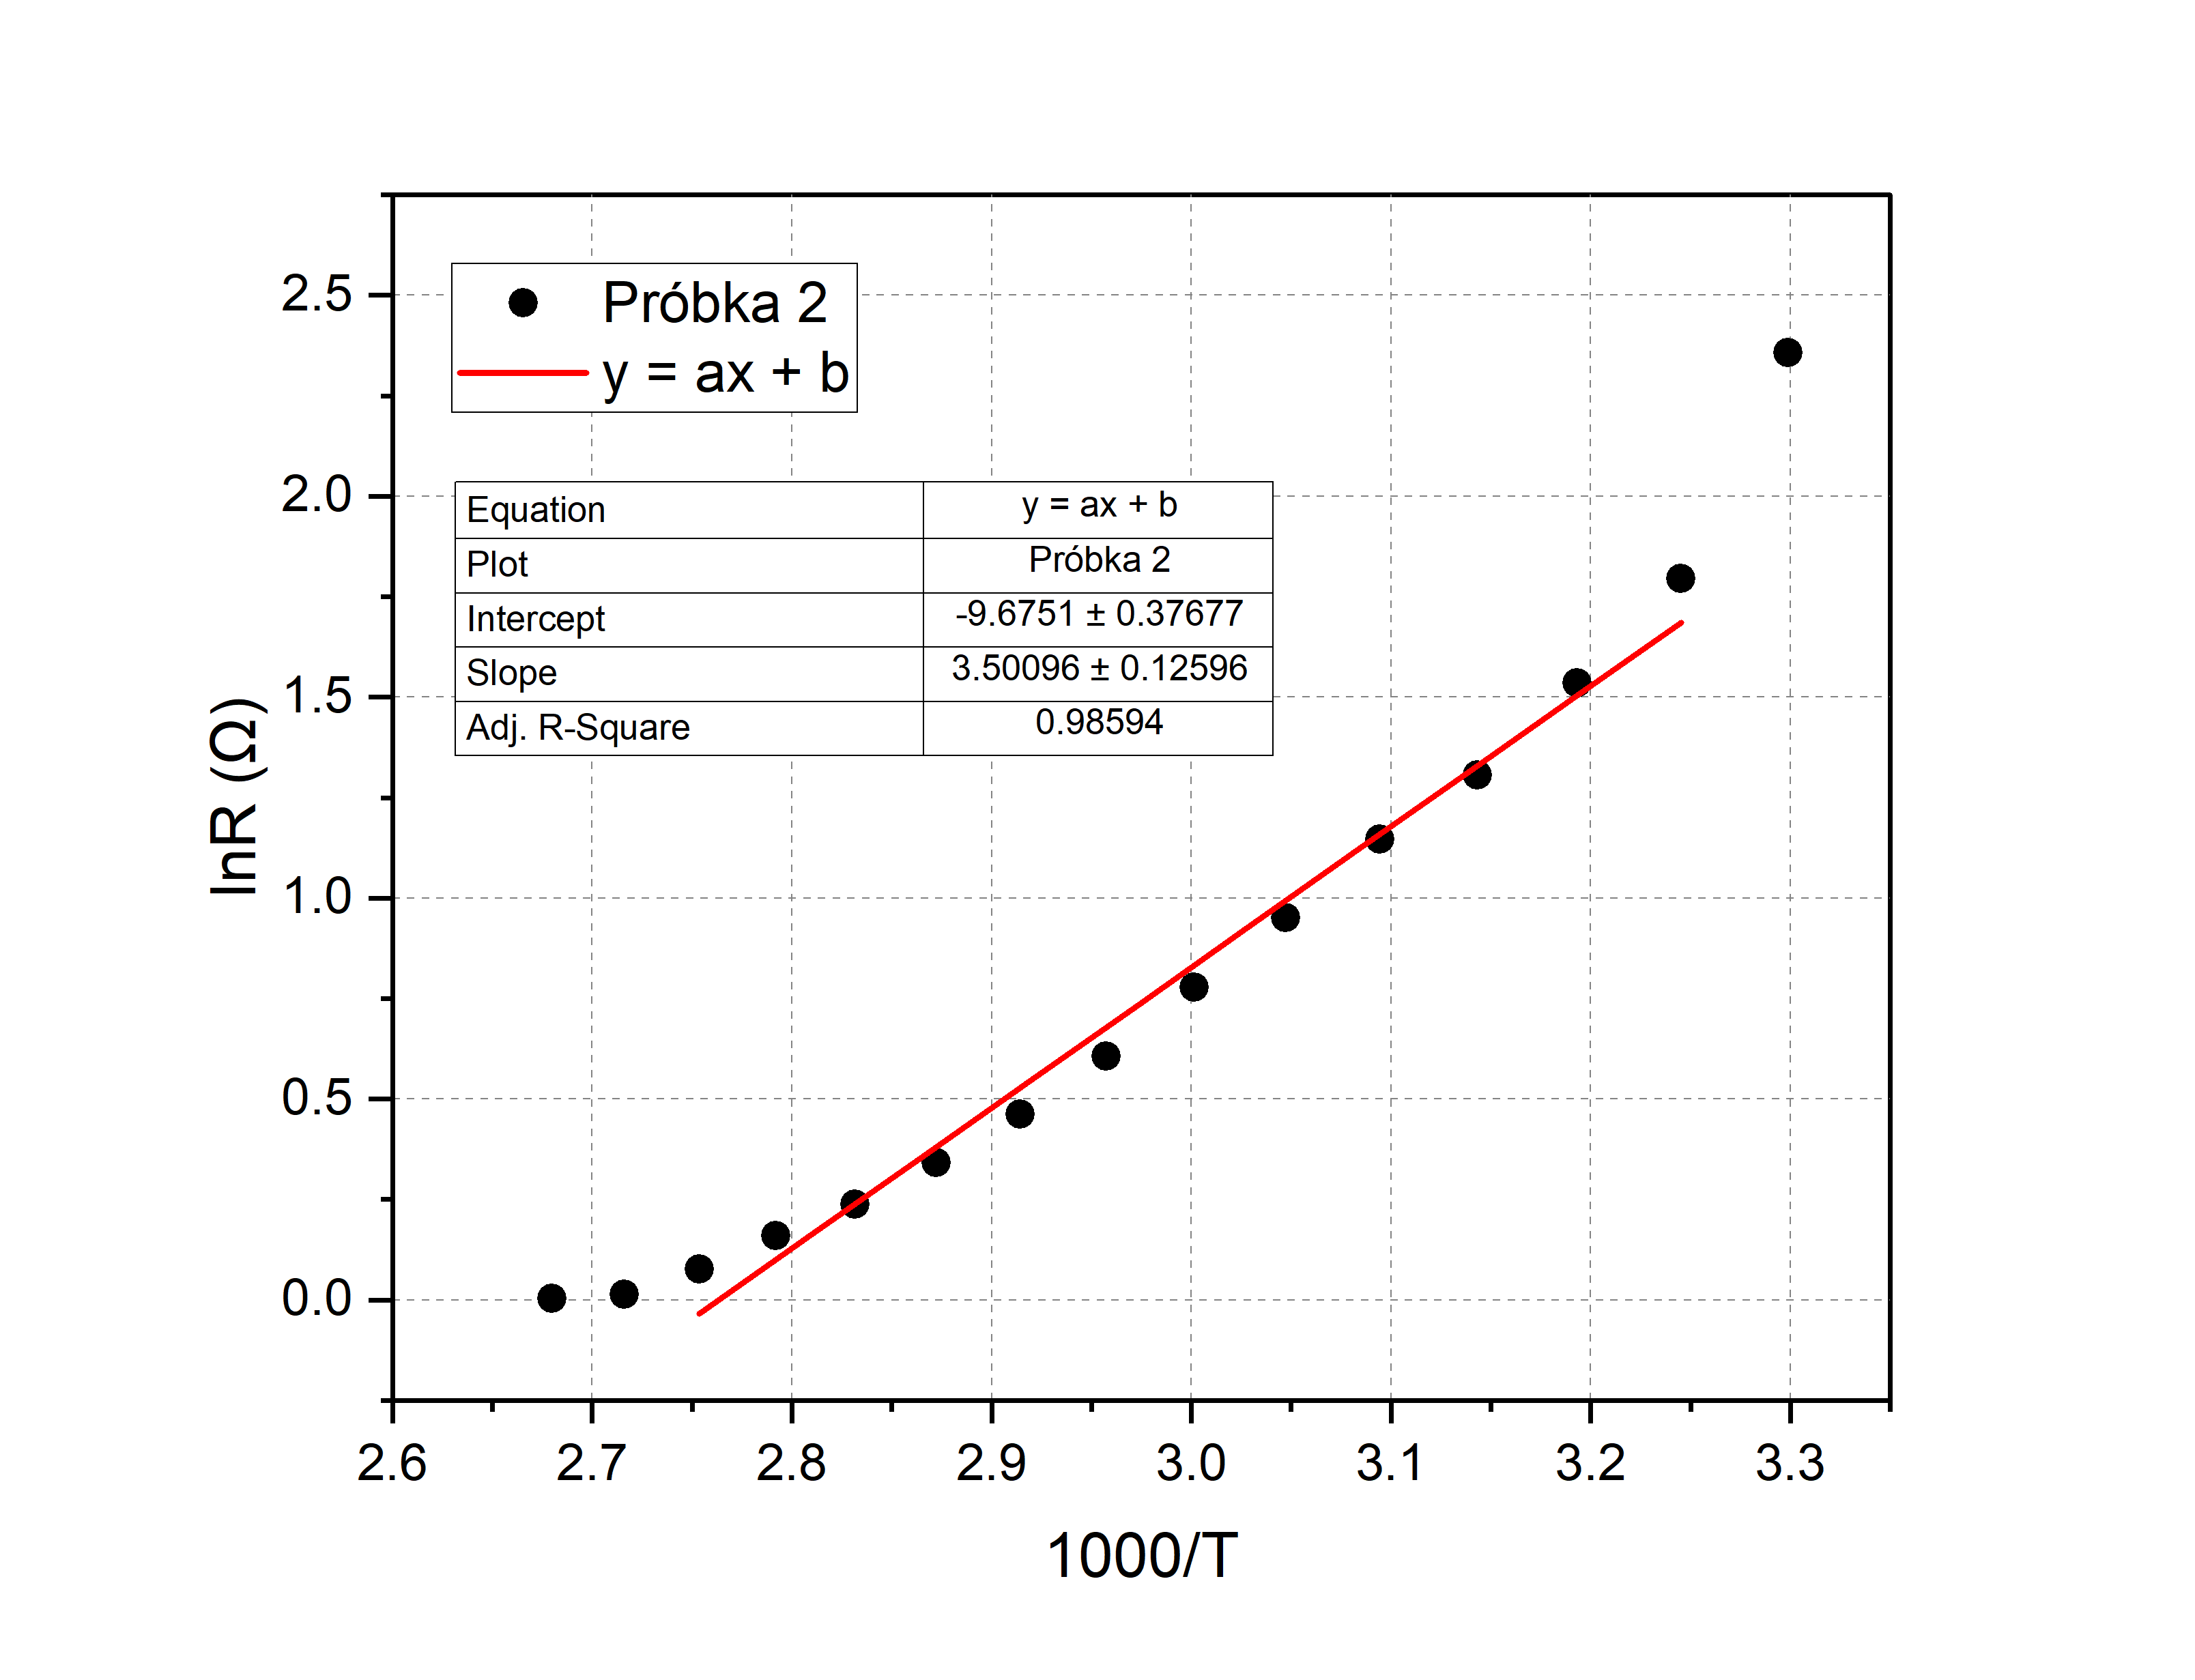
\includegraphics[width = 150mm]{imgs/Graph2.png}
    \caption{Wykres zależności $lnR_s = f(\frac{1000}{T})$ dla próbki nr.2}
    \label{fig:polprzewodnik}
\end{figure}

Podobnie jak w przykładzie z próbką nr.1 spodziewanym wynikiem miała być funkcja liniowa.
Dopasowaliśmy więc prostą do danych otrzymując również 98,6\% dopasowania.

W tym przypadku wzór regresji liniowej $y = ax + b$ ma postać:

$$lnR_s = \frac{E_g}{2k} \frac{1000}{T} \cdot 10^{-3} + lnR_{s,o}$$

Pasmo wzbronione $E_g$ wyznaczymy z porównania współczynnika a regresji liniowej z współczynnikiem kierunkowym funkcji $lnR_s = f(\frac{1000}{T})$:

$$a = \frac{E_g}{2k} \cdot 10^{-3} \Rightarrow 2ak = E_g \cdot 10^{-3} \Rightarrow E_g = 2000ak$$

Wartość k jest stałą Bolzmana i jest równa $k = 1,3806 \cdot 10^{23} \frac{J}{K}$

$$E_g = 2000 \cdot 3,5 \cdot 1,3806 \cdot 10^{-23} \approx 9.66 \cdot 10^{-20}J$$

W tym przypadku również należy obliczyć błąd złożony:

$$u_c^2(E_g) = \displaystyle\sum_{i=1}^{n} \left( \frac{\partial f}{\partial x_i} \right)^2 u^2(x_i) = \left( 2000k \right)^2 u^2(a) \approx 1,21 \cdot 10^{-41} \Rightarrow u_c(E_g) \approx 0,348 \cdot 10^{-20}$$

Wartość końcowa pasma wzbronionego jest równa:

$$E_g = (9.660 \pm 0,348) \cdot 10^{-20}J \approx 0.603 \pm 0.022 eV$$
